\usetikzlibrary{arrows,positioning}
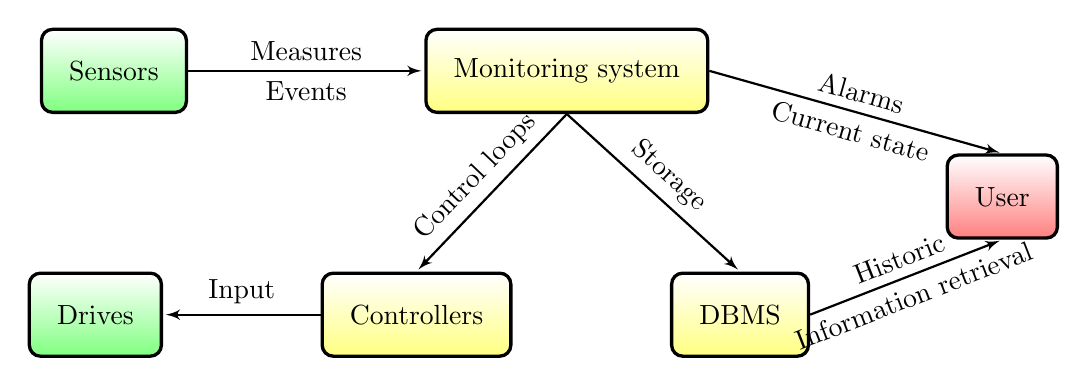
\begin{tikzpicture}[node distance=0.5cm]  
  \tikzset{
    mynode/.style={rectangle,rounded corners,draw=black, 
      very thick, inner sep=1em, minimum size=3em, text centered,
      groc},
    myarrow/.style={->, >=latex', shorten >=1pt, thick},
    mylabel/.style={text width=7em, text centered},
    groc/.style={top color=white, bottom color=yellow!50},
    verd/.style={top color=white, bottom color=green!50},
    roig/.style={top color=white, bottom color=red!50},
  }  

  \node[mynode]                                       (monitor)   {Monitoring system};  
  \node[mynode, below right=2cm and -0.5cm of monitor]  (bd)        {DBMS}; 
  \node[mynode, below=2cm of monitor, left=2cm and 2cm of bd]     (control)   {Controllers}; 
  \node[mynode, roig, below right=0.5cm and 3cm of monitor] (usuari)    {User};  
  \node[mynode, verd, left=2cm of control]            (actuador)  {Drives};
  \node[mynode, verd, left=3cm of monitor]            (sensor)    {Sensors};  


  \draw[myarrow] (monitor.east) --   (usuari.north)	
     node [above,sloped,midway] {Alarms}
     node [below,sloped,midway] {Current state};
  \draw[myarrow] (bd.east) --   (usuari.south)
     node [above,sloped,midway] {Historic}
     node [below,sloped,midway] {Information retrieval};
  \draw[myarrow] (sensor.east) --   (monitor.west) 
     node [above,midway] {Measures}
     node [below,midway] {Events};
  \draw[myarrow] (control.west) -- (actuador.east)
     node [above,midway] {Input};
  \draw[myarrow] (monitor.south) -- (bd.north)
     node [above,sloped,midway] {Storage};
  \draw[myarrow] (monitor.south) -- (control.north)
     node [above,sloped,midway] {Control loops};

\end{tikzpicture} 